% Diese Datei ist Teil des Buchs "Schreibe Dein Programm!"
% Das Buch ist lizensiert unter der Creative-Commons-Lizenz
% "Namensnennung - Weitergabe unter gleichen Bedingungen 4.0 International (CC BY-SA 4.0)"
% https://creativecommons.org/licenses/by-sa/4.0/deed.de

\chapter{Higher-Order-Programmierung}
\label{cha:higher-order}

Der renommierte Informatiker Paul Hudak wurde einst gefragt, was die
drei wichtigsten Dinge beim Programmieren seien.  Er antwortete:
"<Abstraktion, Abstraktion, Abstraktion">.  Entsprechend ist das
Mantra~\ref{mantra:abstraktion} auf Seite~\pageref{mantra:abstraktion}
auch eins der wichtigsten:

\mantraabstraktion*

\noindent In diesem Kapitel werden wir dieses Mantra konsequent anwenden.  Dabei
kommt oft eine besondere Art Funktion heraus: Funktionen, die andere
Funktionen als Eingabe akzeptieren oder als Ausgabe liefern.  Solche
Funktionen heißen auch \textit{Funktionen höherer
  Ordnung}\index{Funktion!höherer Ordnung} oder
\textit{Higher-Order-Funktion}.\index{Higher-Order-Funktion}  Um die
resultierende Art der Programmierung~-- die
\textit{Higher-Order-Programmierung}~-- geht es in diesem Kapitel.

\section{Fußball-Fakten ermitteln}

Eine nahezu unerschöpfliche Quelle für Diskussionen stellen die
Fußballergebnisse dar.  Hier stellen sich so bedeutsame Fragen wie:
\begin{itemize}
\item Wie hat diese Saison Bayern München gegen 1.~FC Kaiserslautern
  auswärts gespielt?\footnote{Wir wissen, das ist schon eine Weile her.}
\item Wie viele Tore sind in dieser Saison gefallen?
\item Welche Mannschaft ist abstiegsgefährdet?
\end{itemize}
%
All diese Informationen speisen sich aus Ergebnissen der Spiele einer
Saison.  Ein Spiel können wir folgendermaßen charakterisieren:
%
\begin{lstlisting}
; Ein Spiel hat folgende Eigenschaften:
; - Spieltag
; - Heimmannschaft
; - Heimmannschaft-Tore
; - Gastmannschaft
; - Gastmannschaft-Tore
\end{lstlisting}
%
Es handelt sich sichtlich um zusammengesetzte Daten.  Wir müssen uns
überlegen, welche Signaturen zu den einzelnen Bestandteilen passen.
Spieltag und Tore sind allesamt natürliche Zahlen.  Eine Mannschaft können
wir durch ihren Namen als Zeichenkette repräsentieren.   Das ergibt
folgende Record-Definition:
%$
\begin{lstlisting}
(define-record game
  make-game game?
  (game-matchday natural)
  (game-home-team string)
  (game-home-goals natural)
  (game-guest-team string)
  (game-guest-goals natural))
\end{lstlisting}
%
Es folgen hier beispielhaft die Ergebnisse des ersten Spieltags der Bundesliga-Saison
2009/2010:
\begin{lstlisting}
(define game1 (make-game 1 "Wolfsburg" 2 "Stuttgart" 0))
(define game2 (make-game 1 "Mainz" 2 "Bayer 04" 2))
(define game3 (make-game 1 "Hertha" 1 "Hannover" 0))
(define game4 (make-game 1 "Bremen" 2 "Frankfurt" 3))
(define game5 (make-game 1 "Nürnberg" 1 "Schalke" 2))
(define game6 (make-game 1 "Dortmund" 1 "1. FC Köln" 0))
(define game7 (make-game 1 "Hoffenheim" 1 "Bayern" 1))
(define game8 (make-game 1 "Bochum" 3 "Gladbach" 3))
(define game9 (make-game 1 "Freiburg" 1 "Hamburg" 1))

(define day1
  (list game1 game2 game3 game4 game5 game6 game7 game8 game9))
\end{lstlisting}
%
% FIXME: actual link
Die kompletten Ergebnisse dieser Saison lassen sich unter dem Namen
\texttt{soccer.rkt} von der Webseite des Buchs~--
\url{https://www.deinprogramm.de/}~-- herunterladen.

Eine recht einfache Frage ist die Bestimmung der Punktzahl, welche die
Gastgebermannschaft in einem bestimmten Spiel erzielt hat.  Die
Punktzahl ist zwar eine natürliche Zahl, es gibt aber nur drei
Möglichkeiten: 0, 1 und 3.  Wir können also eine präzisere Signatur
als \lstinline{points} definieren:
%
\begin{lstlisting}
; Punktzahl in Spiel
(define points
  (signature (enum 0 1 3)))
\end{lstlisting}
%
Unsere Funktion für die Bestimmung der Punktzahl hat Kurzbeschreibung,
Signatur, Tests und Gerüst wie folgt:\index{home-points@\texttt{home-points}}
%
\begin{lstlisting}
; Punktzahl für Heimmannschaft berechnen
(: home-points (game -> points))

(check-expect (home-points game1) 3)
(check-expect (home-points game2) 1)
(check-expect (home-points game3) 3)
(check-expect (home-points game4) 0)

(define home-points
  (lambda (game)
    ...))
\end{lstlisting}
% 
Entsprechend der Signatur der Ausgabe fallen die Spiele in drei
unterschiedliche Klassen, das heißt wir brauchen eine Verzweigung mit
drei Zweigen entsprechend den drei möglichen Punktzahlen:
%
\begin{lstlisting}
(define home-points
  (lambda (game)
    (cond
      (... 3)
      (... 0)
      (... 1))))
\end{lstlisting}
%
Die Bedingungen der drei Zweige kommen aus den Fußballregeln~-- wir
müssen die Tore von Heim- und Gastmannschaft vergleichen:
%
\begin{lstlisting}
(define home-points
  (lambda (game)
    (cond
      ((> (game-home-goals game) (game-guest-goals game)) 3)
      ((< (game-home-goals game) (game-guest-goals game)) 0)
      ((= (game-home-goals game) (game-guest-goals game)) 1))))
\end{lstlisting}
%
Das funktioniert schon korrekt, ist aber noch unelegant.
Das \lstinline{(game-home-goals game)} ist dreimal wiederholt~-- wir
sollten eine lokale Definition einführen, damit es nur einmal
dasteht.  Ebenso für den Aufruf von \lstinline{game-guest-goals}.  Das
sieht dann so aus:\label{func:home-points}
%
\begin{lstlisting}
(define home-points
  (lambda (game)
    (define goals1 (game-home-goals game))
    (define goals2 (game-guest-goals game))
    (cond
      ((> goals1 goals2) 3)
      ((< goals1 goals2) 0)
      ((= goals1 goals2) 1))))
\end{lstlisting}
%
Du könntest berechtigterweise fragen, warum die lokalen Variablen
\lstinline{goals1} und \lstinline{goals2} heißen, und nicht
\lstinline{home-goals} und \lstinline{guest-goals} heißen.  Das wird
bei der nächsten Funktion (hoffentlich) klar, welche die Punkte
ausrechnet, die dem Gästeteam zustehen:
%
\begin{lstlisting}
; Punktzahl für Gastmannschaft berechnen
(: guest-points (game -> points))

(define guest-points
  (lambda (game)
    (define goals1 (game-guest-goals game))
    (define goals2 (game-home-goals game))
    (cond
      ((> goals1 goals2) 3)
      ((< goals1 goals2) 0)
      ((= goals1 goals2) 1))))
\end{lstlisting}
%
Diese beiden Funktionen sind weitgehend identisch, der einzige
Unterschied ist die Definition der lokalen Variablen
\lstinline{goals1} und \lstinline{goals2}. Eine solche Duplizierung
von Code ist immer schlecht, vor allem, wenn sich etwas
ändert. Theoretisch könnte der Fußballbund die Regeln für die Vergabe
von Punkten ändern, und dann müssten wir beide Funktionen in
gleicher Weise anpassen.  Die Lösung für das Problem zeigt sich
dadurch, dass wir aus dem gemeinsamen Code der beiden Funktionen
eine neue Funktion machen, entsprechend dem Abstraktions-Mantra:

\mantraabstraktion*

\noindent Um zu abstrahieren, kopieren wir eine der beiden Funktionsdefinitionen und
geben ihr einen neuen Namen, in diesem Fall \lstinline{compute-points}:
%
\begin{lstlisting}
(define compute-points
  (lambda (game)
    (define goals1 (game-guest-goals game))
    (define goals2 (game-home-goals game))
    (cond
      ((> goals1 goals2) 3)
      ((< goals1 goals2) 0)
      ((= goals1 goals2) 1))))
\end{lstlisting}
%
Nun identifizieren wir in der kopierten Funktion die Stellen, die sich
bei den beiden ursprünglichen Funktionen unterscheiden und ersetzen
diese Stellen durch neue Namen.  Hier sind das gerade
\lstinline{game-guest-goals} und \lstinline{game-home-goals}, wir
ersetzen sie durch die Namen \lstinline{get-goals-1} und
\lstinline{get-goals-2}:
%
\begin{lstlisting}
(define compute-points
  (lambda (game)
    (define goals1 (get-goals-1 game))
    (define goals2 (get-goals-2 game))
    (cond
      ((> goals1 goals2) 3)
      ((< goals1 goals2) 0)
      ((= goals1 goals2) 1))))
\end{lstlisting}
%
Diese neuen Variablen sind noch ungebunden, wir müssen sie deshalb
noch im \lstinline{lambda} unterbringen:
%
\begin{lstlisting}
(define compute-points
  (lambda (get-goals-1 get-goals-2 game)
    (define goals1 (get-goals-1 game))
    (define goals2 (get-goals-2 game))
    (cond
      ((> goals1 goals2) 3)
      ((< goals1 goals2) 0)
      ((= goals1 goals2) 1))))
\end{lstlisting}
%
Damit können wir die bisherigen Definitionen von
\lstinline{home-points} und \lstinline{guest-points} ersetzen durch
die folgenden:
%
\begin{lstlisting}
(define home-points
  (lambda (game)
    (compute-points game-home-goals game-guest-goals game)))

(define guest-points
  (lambda (game)
    (compute-points game-guest-goals game-home-goals game)))
\end{lstlisting}
%
Diese neuen Definitionen lassen die Gemeinsamkeiten und Unterschiede
beider Funktionen klar erkennen und vermeiden die doppelte Definition
der Fußball-Punkteregeln.

\textbf{Wichtig:} Diese beiden Definitionen müssen \emph{nach} der
Definition von \lstinline{compute-points} stehen, da davor
\lstinline{compute-points} noch nicht definiert ist.

Der neuen Funktion fehlt noch eine Signatur.  Die Funktion akzeptiert
drei Argumente.  Das letzte hat die Signatur \lstinline{game}.  Die
ersten beiden werden aus den Funktionen \lstinline{game-home-goals}
und \lstinline{game-guest-goals} bestückt, die jeweils die Signatur
\lstinline{(game -> natural)} haben.  Daraus können wir die Signatur
für \lstinline{compute-points} zusammensetzen:
%
\begin{lstlisting}
(: compute-points ((game -> natural) (game -> natural) game -> points))
\end{lstlisting}
%
In der Signatur tauchen mehrere Pfeile auf, weil die Funktion
\lstinline{compute-points} ihrerseits zwei Funktionen als Argumente
akzeptiert.  Solche Funktionen mit mehreren Pfeilen in der Signatur
heißen \textit{Funktionen höherer Ordnung\index{Funktion!höherer
    Ordnung}} oder
\textit{Higher-Order-Funktionen\index{Higher-Order-Funktion}}.

Die Abstraktion bei der Entwicklung von \lstinline{compute-points}
hätten wir auch etwas anders anstellen können: Wir haben bei
\lstinline{compute-points} die beiden Parameter
\lstinline{get-goals-1} und \lstinline{get-goals-2} zu dem schon
bestehenden \lstinline{lambda} hinzugefügt.  Wir können stattdessen
auch ein neues \lstinline{lambda} einfügen.  (Bei Definitionen, in
denen noch kein \lstinline{lambda} steht, müssten wir das sowieso.)
Das sieht dann so aus:
%
\begin{lstlisting}
(define make-compute-points
  (lambda (get-goals-1 get-goals-2)
    (lambda (game)
      (define goals1 (get-goals-1 game))
      (define goals2 (get-goals-2 game))
      (cond
        ((> goals1 goals2) 3)
        ((< goals1 goals2) 0)
        ((= goals1 goals2) 1)))))
\end{lstlisting}
%
Die Signatur dieser Funktion unterscheidet sich leicht von der
Signatur von \lstinline{compute-points}.  Sie akzeptiert nicht mehr drei
Argumente sondern nur zwei, aber liefert dafür eine Funktion, die von
einem Spiel die Punkte liefert:
%
\begin{lstlisting}
(: make-compute-points ((game -> natural) (game -> natural) 
                         -> (game -> points)))
\end{lstlisting}
%
Auch mit dieser Funktion können wir alternative Definitionen von
\lstinline{make-compute-points} schreiben.  Auf den ersten Blick ist
das umständlich, wenn wir das genauso machen wie mit
\lstinline{compute-points}, da wir noch mehr Klammern brauchen:
%
\begin{lstlisting}
(define home-points
  (lambda (game)
    ((make-compute-points game-home-goals game-guest-goals) game)))

(define guest-points
  (lambda (game)
    ((make-compute-points game-guest-goals game-home-goals) game)))
\end{lstlisting}
%
Vielleicht fällt Dir aber das Muster auf, das diese beiden
Definitionen gemeinsam haben:
%
\begin{lstlisting}
(define f
  (lambda (x)
    (g x)))
\end{lstlisting}
%
Das heißt, wenn das Programm \lstinline{f} aufruft, ruft diese
Funktion direkt \lstinline{g} auf, mit der gleichen Eingabe:
\lstinline{f} und \lstinline{g} sind also äquivalent, und wir könnten
genauso gut schreiben:
%
\begin{lstlisting}
(define f g)
\end{lstlisting}
%
Das gleiche Prinzip können wir auch auf \lstinline{home-points} und
\lstinline{guest-points} anwenden:
%
\begin{lstlisting}
(define home-points
  (make-compute-points game-home-goals game-guest-goals))

(define guest-points
  (make-compute-points game-guest-goals game-home-goals))
\end{lstlisting}
%
Man kann auch schön an der Signatur von
\lstinline{make-compute-points} sehen, dass diese als Resultat eine
Funktion mit Signatur \lstinline{(game -> points)} liefert, das ist
gerade die gewünschte Signatur von \lstinline{home-points} und
\lstinline{guest-points}.

Vielleicht hast Du Dich über den Namen \lstinline{make-compute-points}
gewundert: Während die Funktion \lstinline{compute-points} direkt eine Punktzahl
berechnet, macht \lstinline{make-compute-points} eine Funktion, welche
die Punktzahl berechnet: Darum der Präfix \lstinline{make-}.  Es
handelt sich also um eine Art "<Funktionsfabrik">.

\begin{aufgabeinline}
  Wir hätten das neue \lstinline{lambda} auch unterhalb des alten
  \lstinline{lambda} einfügen können statt oberhalb.  Welche Signatur
  hätte die Funktion \lstinline{make-compute-points} dann?  Warum ist
  das keine so gute Idee?
\end{aufgabeinline}

Die Abstraktionstechnik, die wir für die Konstruktion von
\lstinline{compute-points} und \lstinline{make-compute-points}
verwendet haben, wenden wir in diesem Buch noch öfter an.  Sie
verdient deshalb eine eigene Konstruktionsanleitung:

\begin{konstruktionsanleitung}{Abstraktion}
  \label{ka:abstraktion}
  Wenn Du zwei Definitionen geschrieben hast, die inhaltlich verwandt
  sind und viele Ähnlichkeiten aufweisen, abstrahiere wie folgt:
  %
  \begin{enumerate}
  \item Kopiere eine der beiden Definitionen und gib ihr einen neuen
    Namen.
  \item Ersetze die Stellen, bei denen sich die beiden Definitionen
    unterscheiden, jeweils durch eine neue Variable.
  \item Füge die neuen Variablen als Parameter zum \lstinline{lambda}
    der Definition hinzu oder füge ein neues \lstinline{lambda} mit
    diesen Parametern ein.  Du musst gegebenenfalls rekursive Aufrufe
    der Funktion anpassen.
  \item Schreibe eine Signatur für die neue Funktion.
  \item Ersetze die beiden alten Definitionen durch Aufrufe der neuen
    Definition.
  \end{enumerate}
\end{konstruktionsanleitung}

\section{Higher-Order-Funktionen auf Listen}

Als Nächstes wollen wir herausbekommen, welche Spiele einer Saison
unentschieden ausgingen.  Dazu ist zunächst eine Funktion notwendig,
die feststellt, ob \emph{ein} bestimmtes Spiel unentschieden war:
%
\begin{lstlisting}
; Ist Spiel unentschieden?
(: game-draw? (game -> boolean))

(define game-draw?
  (lambda (g)
    (= 1 (home-points g))))
\end{lstlisting}
%
Die Spiele der Saison liegen in einer Liste, wir schreiben also eine
Funktion, die aus einer Liste von Spielen die
unentschiedenen herausholt.  Kurzbeschreibung, Signatur und Gerüst
folgen der Konstruktionsanleitung für Funktionen auf Listen.
Hier ist die Schablone:\index{drawn-games@\texttt{drawn-games}}
%
\begin{lstlisting}
; Unentschiedene Spiele rausfiltern
(: drawn-games ((list-of game) -> (list-of game)))

(check-expect (drawn-games day1) (list game2 game7 game8 game9))

(define drawn-games
  (lambda (list)
    ...))
\end{lstlisting}
%
Die Funktion hat eine Liste als Eingabe, es kommt also die
entsprechende Schablone zur Anwendung:
%
\begin{lstlisting}
(define drawn-games
  (lambda (list)
    (cond
      ((empty? list) ...)
      ((cons? list)
       ... (first list) ...
       ... (drawn-games (rest list)) ...))))
\end{lstlisting}
%
Der rekursive Aufruf liefert die unentschiedenen Spiele des Rests, wir
müssen also nur noch beim ersten Spiel entscheiden, ob es
unentschieden ausging:
%
\begin{lstlisting}
(define drawn-games
  (lambda (list)
    (cond
      ((empty? list) ...)
      ((cons? list)
       ... (game-draw? (first list)) ...
       ... (drawn-games (rest list)) ...))))
\end{lstlisting}
%
Die Funktion \lstinline{game-draw?} liefert einen booleschen Wert,
den können wir eigentlich nur in eine binäre Verzweigung stecken:
%
\begin{lstlisting}
(define drawn-games
  (lambda (list)
    (cond
      ((empty? list) ...)
      ((cons? list)
       (if (game-draw? (first list))
           ...
           ...)
       ... (drawn-games (rest list)) ...))))
\end{lstlisting}
%
Abhängig davon, ob das Spiel unentschieden ist oder nicht, bringen wir
es im Ergebnis unter:
%
\begin{lstlisting}
(define drawn-games
  (lambda (list)
    (cond
      ((empty? list) empty)
      ((cons? list)
       (if (game-draw? (first list))
           (cons (first list) (drawn-games (rest list)))
           (drawn-games (rest list)))))))
\end{lstlisting}
%
Fertig!

Analog zu \lstinline{drawn-games} schreiben wir als Nächstes eine
Funktion, die alle Spiele aus einer Liste extrahiert, die die Heimmannschaft
gewonnen hat.  Dazu brauchen wir erst einmal eine Funktion analog zu
\lstinline{game-draw?}:
%
\begin{lstlisting}
; Hat die Heimmannschaft gewonnen?
(: home-won? (game -> boolean))

(check-expect (home-won? game1) #t)
(check-expect (home-won? game2) #f)
(check-expect (home-won? game4) #f)

(define home-won?
  (lambda (game)
    (= 3 (home-points game))))
\end{lstlisting}
%
Die Funktion \lstinline{home-won-games} entsteht genau analog zu
\lstinline{drawn-games}.  Am Ende kommt folgendes heraus:
%
\begin{lstlisting}
; Spiele herausfiltern, bei denen die Heimmannschaft gewann
(: home-won-games ((list-of game) -> (list-of game)))

(check-expect (home-won-games day1) (list game1 game3 game6))

(define home-won-games
  (lambda (list)
    (cond
      ((empty? list) empty)
      ((cons? list)
       (if (home-won? (first list))
           (cons (first list)
                 (home-won-games (rest list)))
           (home-won-games (rest list)))))))
\end{lstlisting}
%
Die beiden Funktionen \lstinline{drawn-games} und
\lstinline{home-won-games} sind bis auf den Namen fast identisch.  Der
einzige Unterschied ist, dass an der Stelle von \lstinline{game-draw?}
in der zweiten Funktion \lstinline{home-won?} steht.  Darüber können
wir nach Konstruktionsanleitung~\ref{ka:abstraktion} auf
Seite~\pageref{ka:abstraktion} abstrahieren.  Dazu kopieren wir die
letzte Funktion und denken uns einen neuen Namen aus~-- da es in
beiden Fällen ums "<extrahieren"> geht, nehmen wir
\lstinline{extract-games}:
%
\begin{lstlisting}
(define extract-games
  (lambda (list)
    (cond
      ((empty? list) empty)
      ((cons? list)
       (if (home-won? (first list))
           (cons (first list)
                 (extract-games (rest list)))
                 (extract-games (rest list)))))))
\end{lstlisting}
%
Als Nächstes müssen wir die Stelle, die sich bei beiden Definitionen
unterscheidet (\lstinline{game-draw?} beziehungsweise
\lstinline{home-won?}), durch eine neue Variable bezeichnen.  Die nennen wir
\lstinline{f?}:
%
\begin{lstlisting}
(define extract-games
  (lambda (list)
    (cond
      ((empty? list) empty)
      ((cons? list)
       (if (f? (first list))
           (cons (first list)
                 (extract-games (rest list)))
           (extract-games (rest list)))))))
\end{lstlisting}
%
Als Nächstes müssen wir die neue Variable als Parameter zum
\lstinline{lambda} hinzufügen.  Aufpassen: Die beiden rekursiven
Aufrufe müssen ebenfalls um den Parameter erweitert werden:
%
\begin{lstlisting}
(define extract-games
  (lambda (f? list)
    (cond
      ((empty? list) empty)
      ((cons? list)
       (if (f? (first list))
           (cons (first list)
                 (extract-games f? (rest list)))
                 (extract-games f? (rest list)))))))
\end{lstlisting}
%
(Es ist Geschmackssache, ober der neue Parameter vor oder hinter die
alten kommt.)

Die Funktionsdefinition ist damit fertig, aber wir müssen noch eine
Signatur schreiben.  Wir fangen mit der Signatur von
\lstinline{home-won-games} an und erweitern um den zusätzlichen
Parameter:
%
\begin{lstlisting}
(: extract-games (... (list-of game) -> (list-of game)))
\end{lstlisting}
%
Der zusätzliche Parameter ist \lstinline{f?}, den wir für
\lstinline{game-draw?} und \lstinline{home-won?} eingesetzt haben.
Diese beiden Funktionen haben die Signatur
\lstinline{(game -> boolean)}, das können wir also für die Ellipse
einsetzen:
%
\begin{lstlisting}
(: extract-games ((game -> boolean) (list-of game) -> (list-of game)))
\end{lstlisting}
%
Nun können wir Aufrufe der alten Funktionen durch Aufrufe der neuen
ersetzen.  Wir tun das, indem wir die Testfälle für
\lstinline{drawn-games} und \lstinline{home-won-games} anpassen:
%
\begin{lstlisting}
(check-expect (extract-games game-draw? day1) (list game2 game7 game8 game9))
(check-expect (extract-games home-won? day1) (list game1 game3 game6))
\end{lstlisting}
%
Fertig!

Vielleicht hast Du das Gefühl, das Muster der Funktion
\lstinline{extract-games} schon gesehen zu haben.  In der Tat sieht
die Funktion~\lstinline{live-dillos} in
Abschnitt~\ref{page:live-dillos} auf
Seite~\ref{page:live-dillos} ebenfalls den Funktionen
\lstinline{drawn-games} und \lstinline{home-won-games} sehr ähnlich.
Hier ist sie noch einmal zur Erinnerung:
%
\begin{lstlisting}
(: live-dillos ((list-of dillo) -> (list-of dillo)))

(define live-dillos
  (lambda (dillos)
    (cond
      ((empty? dillos) empty)
      ((cons? dillos)
       (if (dillo-alive? (first dillos))
           (cons (first dillos)
                 (live-dillos (rest dillos)))
           (live-dillos (rest dillos)))))))
\end{lstlisting}
%
Und tatsächlich~-- wenn wir \lstinline{dillos} in \lstinline{list}
umbenennen und den gleichen Abstraktionsprozess wie bei
\lstinline{drawn-games} und \lstinline{home-won-games} durchlaufen,
dann entsteht die identische Funktionsdefinition zu
\lstinline{extract-games}.  Allerdings gibt es dann immer noch einen
Unterschied~-- die Signaturen sind unterschiedlich.
Die Funktion \lstinline{extract-games} kann nur Listen von Spielen
verarbeiten, während \lstinline{live-dillos} eine Liste von
Gürteltieren akzeptiert.  Können auch darüber~-- einmal
\lstinline{game}, das andere Mal \lstinline{dillo}~-- abstrahieren?

Können wir! Dazu sollten wir die Funktion noch umbenennen, wir wählen
\lstinline{extract-list} statt \lstinline{extract-games}.  Vor allem
aber müssen wir die Signatur ändern, die bisher auf \lstinline{game}
abonniert ist.  Auf Signaturebene abstrahieren wir durch
Signaturvariablen und ersetzen einfach mal probehalber jedes
\lstinline{game} durch \lstinline{%a}:
%
\begin{lstlisting}
(: extract-list ((%a -> boolean) (list-of %a) -> (list-of %a)))
\end{lstlisting}
%
Diese Funktion können wir nun versuchen zu verstehen: Sie akzeptiert
eine Liste von \lstinline{%a}s und eine Funktion, die \lstinline{%a}s
akzeptiert.  Man kann daran fast schon sehen, was die Funktion macht:
Das einzige, was sie mit der Funktion anfangen kann, ist sie auf die
Elemente der Liste anzuwenden~-- sonst gibt es ja weit und breit keine
anderen \lstinline{%a}s.  Dass die Funktion einen booleschen Wert
produziert, suggeriert schon, dass anhand dieses Werts unterschieden
wird.  Die Signatur liefert also wertvolle Informationen darüber, was
die Funktion macht~-- wenn auch nicht alle.
%
\begin{aufgabeinline}
  Schreibe eine andere sinnvolle Funktion mit der gleichen Signatur
  wie \lstinline{extract-list}!
\end{aufgabeinline}
%
Wir betrachten noch eine weitere Anwendung von
\lstinline{extract-list}: Wir wollen aus einer Liste von Spielen die
Spiele extrahieren, an denen eine bestimmte Mannschaft teilgenommen
hat.  Auch dazu definieren wir eine Hilfsfunktion, die feststellt, ob
eine Mannschaft bei einem Spiel die Heim- oder die Gastmannschaft ist:\label{func:plays-game}
%
\begin{lstlisting}
; Spielt Mannschaft bei Spiel?
(: plays-game? (team game -> boolean))

(check-expect (plays-game? "Wolfsburg" game1) #t)
(check-expect (plays-game? "Stuttgart" game1) #t)
(check-expect (plays-game? "Hannover" game1) #f)

(define plays-game?
  (lambda (team game)
    (or (string=? team (game-home-team game))
        (string=? team (game-guest-team game)))))
\end{lstlisting}
%
Nehmen wir an, wir wollen alle Spiele mit Beteiligung von Nürnberg
extrahieren, indem wir \lstinline{extract-list} verwenden.  Um
\lstinline{extract-list} zu verwenden, brauchen wir eine Funktion mit
Signatur~\lstinline{(game -> boolean)}.  Die können wir folgendermaßen
definieren:
%
\begin{lstlisting}
; Spielt Nürnberg mit?
(: plays-nürnberg? (game -> boolean))

(check-expect (plays-nürnberg? game1) #f)
(check-expect (plays-nürnberg? game5) #t)

(define plays-nürnberg?
  (lambda (game)
    (plays-game? "Nürnberg" game)))
\end{lstlisting}
%
Damit können wir zum Beispiel alle Nürnberg-Spiele aus der Saison
extrahieren:
%
\begin{lstlisting}
(extract-list plays-nürnberg? season-2009/2010)
\end{lstlisting}
%
Soweit so gut.  Aber was, wenn wir auch die Spiele des HSV extrahieren
wollen?  Wir könnten eine Funktion \lstinline{plays-hamburg?}
definieren, aber wenn wir viele solcher Anfragen stellen, wird es auf
Dauer umständlich, für jeden Verein extra eine Definiton zu schreiben.

Einfacher ist es, stattdessen die Funktion, die wir an
\lstinline{extract-list} übergeben, "<ad hoc"> mit einem
\lstinline{lambda} zu konstruieren:\label{code:extract-list-plays-game}
%
\begin{lstlisting}
(extract-list (lambda (game) (plays-game? "Nürnberg" game)) 
              season-2009/2010)
(extract-list (lambda (game) (plays-game? "Hamburg" game)) 
              season-2009/2010)
\end{lstlisting}
%
Wir sind von der Signatur her vorgegangen: \lstinline{extract-list}
erwartet eine Funktion mit einem Parameter der Signatur
\lstinline{game}, also schreiben wir ein \lstinline{lambda} mit einem
entsprechenden Parameter.  Wir wollen alle Spiele extrahieren, bei
denen Nürnberg beziehungsweise Hamburg dabei ist, also schreiben wir
den entsprechenden Ausdruck in den Rumpf.
%
\begin{aufgabeinline}
  Schreibe eine Funktion \lstinline{games-playing}, die alle Spiele
  aus einer Liste extrahiert, bei denen eine bestimmte Mannschaft dabei war.
\end{aufgabeinline}
%
Die Funktion \lstinline{extract-list} ist so praktisch, dass sie unter
dem Namen \lstinline{filter}\index{filter@\texttt{filter}} fest
eingebaut ist.

\section{Listen umwandeln}

Bestimmte Fußballstatistiken beschäftigen sich damit, wieviele Tore in
einem Spiel, an einem Spieltag oder in einer ganzen Saison geschossen
wurden.  Grundlage dafür ist die Anzahl Tore eines einzelnen Spiels.
Hier sind Kurzbeschreibung, Signatur, Tests und Gerüst dafür:
%
\begin{lstlisting}
; Gesamttore eines Spiels berechnen
(: total-goals (game -> natural))

(check-expect (total-goals game1) 2)
(check-expect (total-goals game2) 4)

(define total-goals
  (lambda (game)
    ...))
\end{lstlisting}
%
Als Schablone machen wir davon Gebrauch, dass die Eingabe
zusammensetzte Daten sind:
%
\begin{lstlisting}
(define total-goals
  (lambda (game)
    ... (game-matchday game) ...
    ... (game-home-team game) ...
    ... (game-home-goals game) ...
    ... (game-guest-team game) ...
    ... (game-guest-goals game) ...))
\end{lstlisting}
%
Für die Gesamt-Torzahl benötigen wir nur
\lstinline{(game-home-goals game)}
und
\lstinline{(game-guest-goals game)}, die addiert werden:
%
\begin{lstlisting}
(define total-goals
  (lambda (game)
    (+ (game-home-goals game)
       (game-guest-goals game))))
\end{lstlisting}
%
Als Nächstes wollen wir die Gesamttore jeweils aller Spiele eines
Spieltags herausbekommen.  Dazu wollen wir aus einer Liste der Spiele
eine Liste der zugehörigen Gesamttore machen:
%
\begin{lstlisting}
; Gesamttore in einer Liste von Spielen berechnen
(: list-total-goals ((list-of game) -> (list-of natural)))
\end{lstlisting}
%
Das erste Element des Ergebnisses soll die Toranzahl des ersten Spiels
der Eingabeliste sein, das zweite Element die Toranzahl des zweiten
Spiels undsoweiter.  Dieser Test illustriert die Funktionsweise:
%
\begin{lstlisting}
(check-expect (list-total-goals day1)
              (list 2 4 1 5 3 1 2 6 2))
\end{lstlisting}
%
Es folgt das Gerüst mit der obligatorischen Schablone für Funktionen
auf Listen:
%
\begin{lstlisting}
(define list-total-goals
  (lambda (list)
    (cond
      ((empty? list) ...)
      ((cons? list)
       ... (first list)
       ... (list-total-goals (rest list)) ...))))
\end{lstlisting}
%
Falls die Eingabe eine leere Liste ist, so kann auch die Ausgabe nur
leer sein.  Im anderen Zweig steht in der Schablone das erste Spiel:
von dem muss die Funktion die Toranzahl ermitteln, für den Rest ist
das schon passiert.  Die beiden Ergebnisse kombinieren wir mit
\lstinline{cons}:
%
\begin{lstlisting}
(define list-total-goals
  (lambda (list)
    (cond
      ((empty? list) empty)
      ((cons? list)
       (cons (total-goals (first list))
             (list-total-goals (rest list)))))))
\end{lstlisting}
%
\begin{aufgabeinline}
  Benutze die Funktion \lstinline{list-sum} aus
  Abschnitt~\ref{sec:list-sum} auf Seite~\pageref{sec:list-sum}, um
  eine Funktion zu schreiben, welche die durchschnittliche Toranzahl
  einer Liste von Spielen berechnet.
\end{aufgabeinline}
%
Fans sind vielleicht weniger an Gesamttoren interessiert als an den
Toren ihrer Mannschaft.  Damit wir uns da einen Überblick verschaffen
können, benötigen wir wieder erst einmal eine Funktion, welche für ein
einzelnes Spiel die Anzahl der Tore einer bestimmten Mannschaft berechnet:
%
\begin{lstlisting}
; Tore einer Mannschaft aus einem Spiel berechnen
(: team-goals (team game -> natural))

(check-expect (team-goals "Wolfsburg" game1) 2)
(check-expect (team-goals "Stuttgart" game1) 0)
\end{lstlisting}
%
Was soll passieren, wenn die gewünschte Mannschaft bei dem Spiel gar nicht
dabei war?  Das sollte zu einem Fehler führen:
%
\begin{lstlisting}
(check-error (team-goals "Hannover" game1))
\end{lstlisting}
%
Gerüst und Schablone machen zunächst wieder davon Gebrauch, dass es
sich bei \lstinline{game} zum zusammengesetzte Daten handelt:
%
\begin{lstlisting}
(define team-goals
  (lambda (team game)
    ... (game-matchday game) ...
    ... (game-home-team game) ...
    ... (game-home-goals game) ...
    ... (game-guest-team game) ...
    ... (game-guest-goals game) ...))
\end{lstlisting}
%
Außerdem gibt es eine Fallunterscheidung in den Daten, je nachdem, ob
die gesuchte Mannschaft die Heim- oder die Gastmannschaft ist, was zu
einer Verzweigung mit zwei Zweigen führt:
%
\begin{lstlisting}
(define team-goals
  (lambda (team game)
    (cond
      ((string=? team (game-home-team game))
       (game-home-goals game))
      ((string=? team (game-guest-team game))
       (game-guest-goals game)))))
\end{lstlisting}
%
Jetzt wollen wir auch diese Funktion benutzen, um eine ganze Liste von
Spielen, bei denen eine bestimmte Mannschaft mitspielt, in die Liste
der Tore dieser Mannschaft verwandelt.  Signatur und Kurzbeschreibung
sehen so aus:
%
\begin{lstlisting}
; Tore einer Mannschaft aus einer Liste von Spielen auflisten
(: list-team-goals (team (list-of game) -> (list-of natural)))
\end{lstlisting}
%
\begin{aufgabeinline}
  Schreibe einen Testfall, der eine Liste der Tore von Hamburg in
  einer Saison berechnet.  Benutze dazu \lstinline{filter}! 
\end{aufgabeinline}
%
Gerüst und Schablone sehen so aus:
%
\begin{lstlisting}
(define list-team-goals
  (lambda (team list)
    (cond
      ((empty? list) ...)
      ((cons? list)
      ... (first list) ...
      ... (list-team-goals team (rest list)) ...))))
\end{lstlisting}
%
Und wieder kommt bei einer leeren Liste als Eingabe eine leere Liste
heraus, und wir wenden im \lstinline{cons}-Fall die zuvor geschriebene
Hilfsfunktion auf das erste Element an und bauen mit \lstinline{cons}
die Ergebnis-Liste:
%
\begin{lstlisting}
(define list-team-goals
  (lambda (team list)
    (cond
      ((empty? list) empty)
      ((cons? list)
       (cons (team-goals team (first list))
             (list-team-goals team (rest list)))))))
\end{lstlisting}
%
Fertig!

Allerdings ruft mal wieder das Abstraktions-Mantra: Die Funktionen
\lstinline{list-total-goals} und \lstinline{list-team-goals} ähneln
sich stark.  Sie unterscheiden sich nur darin, dass bei der ersten
\lstinline{total-goals} auf dem ersten Element der Liste auferufen wird
und beim zweiten \lstinline{team-goals}. 

Um zu abstrahieren, gehen wir wieder nach
Konstruktionsanleitung~\ref{ka:abstraktion} auf
Seite~\pageref{ka:abstraktion} vor.  Wir kopieren eine der beiden
Funktionen (wir nehmen die erste) und geben ihr einen neuen Namen:
%
\begin{lstlisting}
(define list-apply
  (lambda (list)
    (cond
      ((empty? list) empty)
      ((cons? list)
       (cons (total-goals (first list))
             (list-apply (rest list)))))))
\end{lstlisting}
%
Die Funktion heißt \lstinline{list-apply}, weil sie eine Funktion auf
alle Elemente einer Liste anwendet.

Als Nächstes müssen wir eine Variable dort einführen, wo die beiden
Funktionen sich unterscheiden, nämlich bei \lstinline{total-goals}.
Wir nennen die Funktion einfach \lstinline{f}:
%
\begin{lstlisting}
(define list-apply
  (lambda (list)
    (cond
      ((empty? list) empty)
      ((cons? list)
       (cons (f (first list))
             (list-apply (rest list)))))))  
\end{lstlisting}
%
Nun müssen wir die neue Variable noch im \lstinline{lambda}
unterbringen, ohne zu vergessen, sie auch im rekursiven Aufruf
aufzuführen:
%
\begin{lstlisting}
(define list-apply
  (lambda (f list)
    (cond
      ((empty? list) empty)
      ((cons? list)
       (cons (f (first list))
             (list-apply f (rest list)))))))
\end{lstlisting}
%
\begin{aufgabeinline}
  Ändere die Definition von \lstinline{list-total-goals} so, dass sie
  \lstinline{list-apply} benutzt.
\end{aufgabeinline}
%
Wir brauchen noch eine Signatur für die neue Funktion.  Wir versuchen
sie mal, "<von null"> zu konstruieren, indem wir aufschreiben, was wir
wissen.  Wir wissen, dass \lstinline{list-apply} zwei Argumente hat,
von denen das erste eine einstellige Funktion und das zweite eine
Liste ist.  Außerdem produziert die Funktion auch eine Liste als
Ergebnis.  Das sieht schriftlich so aus:
%
\begin{lstlisting}
(: list-apply ((... -> ...) (list-of ...) -> (list-of ...)))
\end{lstlisting}
%
Wir haben zwar über zwei Funktionen abstrahiert, die sich mit Spielen
beschäftigt.  Aber \lstinline{list-apply} hat nichts
Fußball-spezifisches mehr an sich.  Wir wissen also nichts über die
Signatur der Elemente der Eingabeliste.  Wir schreiben dort also eine
Signaturvariable hin:
%
\begin{lstlisting}
(: list-apply ((... -> ...) (list-of %element) -> (list-of ...)))
\end{lstlisting}
%
Nun wissen wir, dass die Elemente der Eingabeliste als Eingabe für die
Funktion \lstinline{f} verwendet werden, wir können also auch dort
\lstinline{%element} hinschreiben:
%
\begin{lstlisting}
(: list-apply ((%element -> ...) (list-of %element) -> (list-of ...)))
\end{lstlisting}
%
Die Definition von \lstinline{list-apply} legt auch für das Ergebnis
von  \lstinline{f} keine Signatur fest.  Wir schreiben also auch da
eine Signaturvariable hin:
%
\begin{lstlisting}
(: list-apply ((%element -> %result) (list-of %element) -> (list-of ...)))
\end{lstlisting}
%
Es fehlt nur noch die Signatur für die Elemente der Ergebnisliste.
Dafür müssen wir den Aufruf von \lstinline{cons} betrachten, dessen
erstes Argument gerade das Ergebnis des Aufrufs von \lstinline{f}
ist.  Dort muss deshalb auch \lstinline{%result} hin:
%
\begin{lstlisting}
(: list-apply ((%element -> %result) (list-of %element) -> (list-of %result)))
\end{lstlisting}
%
Bei solchen Signaturen, in denen überhaupt nichts über die
Signaturvariablen bekannt ist, ist es üblich, kürzere Namen für die
Signaturvariablen zu wählen, zum Beispiel so:
%
\begin{lstlisting}
(: list-apply ((%a -> %b) (list-of %a) -> (list-of %b)))
\end{lstlisting}
%
Fertig!
%
\begin{aufgabeinline}
  Schreibe auch \lstinline{list-team-goals} so um, dass es
  \lstinline{list-apply} verwendet.  Du musst einen ähnlichen Trick
  verwenden wie bei der Kombination von \lstinline{extract-list} und
  \lstinline{plays-game?} im vorigen Abschnitt auf
  Seite~\pageref{code:extract-list-plays-game}.
\end{aufgabeinline}
%
Die Funktion \lstinline{list-apply} ist ähnlich praktisch wie
\lstinline{filter} aus dem vorigen Abschnitt und ist darum unter dem
Namen \lstinline{map} fest eingebaut.\index{map@\texttt{map}}

\section{Listen zusammenfalten}
\label{sec:fold}

In Abschnitt~\ref{sec:list-sum} haben wir auf
Seite~\pageref{sec:list-sum} die Funktionen \lstinline{list-sum} und
\lstinline{list-product} geschrieben, welche die Summe einer Liste von
Zahlen bildet:
%
\begin{lstlisting}
; Summe der Elemente einer Liste von Zahlen berechnen
(: list-sum ((list-of number) -> number))

(define list-sum
  (lambda (list)
    (cond
      ((empty? list) 0)
      ((cons? list)
       (+ (first list) (list-sum (rest list)))))))

; Produkt der Elemente einer Liste von Zahlen berechnen
(: list-product (list-of-numbers -> number))

(define list-product
  (lambda (list)
    (cond
      ((empty? list) 1)
      ((cons? list)
       (* (first list) (list-product (rest list)))))))
\end{lstlisting}
%
Die Definitionen von \lstinline{list-sum} und \lstinline{list-product}
unterscheiden sich, bis auf den Namen, nur an zwei Stellen: im Zweig
für \lstinline{empty}, wo das jeweilige neutrale Element steht, und im
Zweig für \lstinline{cons}, wo die Funktion steht, die benutzt wird,
um das erste Element mit dem Ergebnis des rekursiven Aufrufs zu
kombinieren.  Es ist also eine gute Idee zu abstrahieren!

Wir gehen wieder nach Konstruktionsanleitung~\ref{ka:abstraktion} auf
Seite~\pageref{ka:abstraktion} vor.  Uns ist beim ersten Mal, als wir
das gemacht haben, kein guter Name eingefallen.  Das ist keine
Schande: Wir fangen deshalb mit \lstinline{xxx} an in der Hoffnung,
dass uns später ein besserer Name einfällt:
%
\begin{lstlisting}
(define xxx
  (lambda (list)
    (cond
      ((empty? list) 1)
      ((cons? list)
       (* (first list) (xxx (rest list)))))))
\end{lstlisting}
%
Als Nächstes müssen wir die Unterschiede zwischen den beiden
Funktionen durch neue Variablen ersetzen, das sind hier gerade
\lstinline{1} und \lstinline{*}.  Die neuen Variablen nennen wir
\lstinline{for-empty} und \lstinline{for-cons}, weil sie in den
Zweigen für \lstinline{empty} respektive \lstinline{cons} stehen:
%
\begin{lstlisting}
(define xxx
  (lambda (list)
    (cond
      ((empty? list) for-empty)
      ((cons? list)
       (for-cons (first list) (xxx (rest list)))))))
\end{lstlisting}
%
Für den nächsten Schritt fügen wir die neuen Variablen zum bestehenden
\lstinline{lambda} hinzu.  Wir müssen wieder darauf achten, die
Variablen auch zum rekursiven Aufruf hinzuzufügen:
%
\begin{lstlisting}
(define xxx
  (lambda (for-empty for-cons list)
    (cond
      ((empty? list) for-empty)
      ((cons? list)
       (for-cons (first list)
                 (xxx for-empty for-cons (rest list)))))))
\end{lstlisting}
%
Diese Funktion kann sowohl die Aufgabe von \lstinline{list-sum} als
auch die von \lstinline{list-product} erledigen:
%
\begin{lstlisting}
(xxx 0 + (list 1 2 3 4))
|\evalsto| 10
\end{lstlisting}
%
und so aufmultiplizieren:
%
\begin{lstlisting}
(xxx 1 * (list 1 2 3 4))
|\evalsto| 24
\end{lstlisting}
%
Als Nächstes steht nach Konstruktionsanleitung die Signatur für die
neue Funktion an.  Es liegt nahe, die Signatur von
\lstinline{list-sum} beziehungsweise \lstinline{list-product} zu
verallgemeinern.  Für den neuen Parameter \lstinline{for-empty}
verwenden wir die Signatur von \lstinline{0} und \lstinline{1}, also
\lstinline{number}.  Für \lstinline{for-cons} verwenden wir die
Signatur von \lstinline{+} und \lstinline{*}, also
\lstinline{(number number -> number)}:
%
\begin{lstlisting}
(: xxx (number (number number -> number) (list-of number) -> number))
\end{lstlisting}
%
Bei näherer Betrachtung steht aber in der Definition von
\lstinline{xxx} allerdings nichts "<zahlenspezifisches">, wir könnten
also versuchen, \lstinline{number} durch eine Signaturvariable zu
ersetzen, wie wir es auch bei \lstinline{list-apply} bzw. \lstinline{map} im vorigen
Abschnitt gemacht haben:
%
\begin{lstlisting}
(: xxx (%a (%a %a -> %a) (list-of %a) -> %a))
\end{lstlisting}
%
Das heißt, wir könnten versuchen, \lstinline{xxx} mit etwas
aufzurufen, das keine Liste von Zahlen ist.  Wir brauchen dafür ein
passendes zweites Argument, also eine
Funktion, deren Signatur die Form \lstinline{(%a %a -> %a)} hat.  Ein
Beispiel ist die Funktion \lstinline{append}, die zwei Listen
aneinanderhängt und folgende Signatur hat:
%
\begin{lstlisting}
((list-of %element) (list-of %element) -> (list-of %element))
\end{lstlisting}
% 
Weil wir \lstinline{(list-of %element)} für \lstinline{%a} einsetzen,
brauchen wir als weitere Argumente für \lstinline{xxx} noch eine
Liste als erstes Argument und eine Liste von Listen als drittes
Argument.  Das könnte so aussehen:
%
\begin{lstlisting}
(xxx empty append (list (list 1 2 3) (list 4 5 6) (list 7 8 9)))
|\evalsto| #<list 1 2 3 4 5 6 7 8 9>
\end{lstlisting}
%
Wir können also \lstinline{xxx} benutzen, um eine Liste von Listen
"<flachzuklopfen">.

Aber ist das schon die beste Signatur für \lstinline{xxx}?  Wir können
wie bei \lstinline{list-map} untersuchen, ob die \lstinline{%a}s
tatsächlich alle gleich sein müssen.  Um das herauszubekommen, könnten
wir mal annehmen, sie seien alle verschieden:
  %
\begin{lstlisting}
(: xxx (%a (%b %c -> %d) (list-of %e) -> %f))
\end{lstlisting}
%
Wenn wir aber die Definition von \lstinline{xxx} genau anschauen, dann
sehen wir, dass jeweils einige Signaturvariablen gleich sein müssen:
%
\begin{itemize}
\item Die Signatur \lstinline{%a} von \lstinline{for-empty} muss die
  gleiche sein wie \lstinline{%f}, weil \lstinline{for-empty} als
  Ergebnis von \lstinline{xxx} verwendet wird.
\item Die Signatur \lstinline{%b} des ersten Arguments von
    \lstinline{for-cons} muss die gleiche sein wie die der
    Listenelemente \lstinline{%a}, weil als erstes Argument
      \lstinline{(first list)} verwendet wird.
\item Die Signatur \lstinline{%c} des Arguments von
    \lstinline{for-cons} muss die gleiche sein wie \lstinline{%f},
     weil das Ergebnis von \lstinline{xxx} dort verwendet wird.
\item Die Signatur \lstinline{%d} des Ergebnisses von
    \lstinline{for-cons} muss ebenfalls die gleiche sein wie
    \lstinline{%f}, weil der Aufruf von \lstinline{for-cons} als
    Ergebnis von \lstinline{xxx} verwendet wird.
\end{itemize}
%
Aber immerhin müssen \lstinline{%a} und \lstinline{%b} nicht gleich
sein.  Es bleibt:
%
\begin{lstlisting}
(: xxx (%a (%b %a -> %a) (list-of %b) -> %a))
\end{lstlisting}
%
\begin{aufgabeinline}
  Verfolge die Auswertung von
\begin{lstlisting}
(xxx 0 + (list 1 2 3))
\end{lstlisting}
  im Stepper!
\end{aufgabeinline}
%
Im Stepper kannst Du sehen, dass \lstinline{xxx} folgendermaßen
arbeitet:
%%HK Ich denke, der Name list-fold kommt erst ein paar Zeilen später
%%an der richtigen Stelle
%
\begin{lstlisting}
(xxx $e$ $c$ #<list $a_1$ $\ldots$ $a_n$ >)
|\evalsto|$\ldots$|\evalsto|
($c$ $a_1$ ($c$ $a_2$ ($\ldots$ ($c$ $a_n$ $u$) $\ldots$)))
\end{lstlisting}
%
Im Fall von \lstinline{0} und \lstinline{+} wird die Liste dann zu
einem einzelnen Wert reduziert oder "<zusammengefaltet">, weswegen wir
die Funktion \lstinline{list-fold} nennen.

Die Funktionsweise von \lstinline{list-fold} können wir daran
veranschaulichen, dass sich die ursprüngliche Liste auch als
%
\begin{lstlisting}
(cons |\(a_1\)| (cons |\(a_2\)| (|\(\ldots\)| (cons |\(a_n\)| empty |\(\ldots\)|)))
\end{lstlisting}
%
schreiben lässt.  Das heißt, an die Stelle von \lstinline{cons} tritt
$c$ und an die Stelle von \lstinline{empty} tritt $e$.

\begin{aufgabeinline}
  Kannst Du daraus ableiten, was hierbei herauskommt, ohne DrRacket zu
  benutzen?
  %
\begin{lstlisting}
(list-fold empty cons (list 1 2 3))
\end{lstlisting}
\end{aufgabeinline}
%
Eine andere, praktische Darstellung von 
\lstinline{list-fold} ist, die Gleichung mit dem Operator
\emph{zwischen} den Operanden zu schreiben (und nicht davor). Um das
deutlich zu machen, schreiben wir für \lstinline{for-cons} nicht $c$
sondern $\odot$:
%
\begin{lstlisting}
(list-fold |\(c\)| |\(\odot\)| #<list |\(a_1\)| |\(\ldots\)| |\(a_n\)|>) 
|\evalsto|$\ldots$|\evalsto|
|\(a_1 \odot (a_2 \odot (\ldots (a_n \odot e)\ldots ))\)|
\end{lstlisting}
%
Die Funktion \lstinline{list-fold} ist erstaunlich vielseitig und kann
die Aufgaben vieler anderer Funktionen auf Listen erledigen.  Zum
Beispiel können wir uns \lstinline{list-apply} noch einmal vorknöpfen
und versuchen, die Definition mit \lstinline{list-fold} zu
schreiben.  Hier zur Erinnerung die bisherige Fassung:
%
\begin{lstlisting}
(define list-apply
  (lambda (f list)
    (cond
      ((empty? list) empty)
      ((cons? list)
       (cons (f (first list))
             (list-apply f (rest list)))))))
\end{lstlisting}
%
Wir wollen \lstinline{list-apply} in folgende Form umschreiben:
%
\begin{lstlisting}
(define list-apply
  (lambda (f list)
    (list-fold ...
               ...
               list)))
\end{lstlisting}
%
Wir müssen passende Werte für die beiden Parameter von
\lstinline{list-fold} finden, \lstinline{for-empty} und
\lstinline{for-cons}.  In \lstinline{list-apply} steht im
\lstinline{empty}-Zweig \lstinline{empty}.

Bei \lstinline{for-cons} ist es nicht so offensichtlich.  Wir können
uns aber an der Signatur orientieren.  Gefragt ist eine Funktion mit
zwei Argumenten: das erste ist das erste Listenelement, das zweite das
Resultat des rekursiven Aufrufs.  Wir können also so anfangen:
%
\begin{lstlisting}
(define list-apply
  (lambda (f list)
    (list-fold empt
               (lambda (first-list result)
                 ...)
               list)))
\end{lstlisting}
%
Im Rumpf des neuen \lstinline{lambda} müssen wir nun Code
hinschreiben, der dem Code aus \lstinline{list-apply} im
\lstinline{cons}-Zweig entspricht, also:
%
\begin{lstlisting}
       (cons (f (first list))
             (list-apply f (rest list)))
\end{lstlisting}
%
Allerdings müssen wir die Parameter aus dem \lstinline{lambda}
benutzen, also \lstinline{first-list} und \lstinline{result}:
\lstinline{first-list} ist gerade der Wert von
\lstinline{(first-lits)}, \lstinline{result} das Resultat des
rekursiven Aufrufs.  Wir ersetzen also "<rückwärts">:
%
\begin{lstlisting}
(define list-apply
  (lambda (f list)
    (list-fold empty
               (lambda (first-list result)
                 (cons (f first-list)
                       result))
               list)))
\end{lstlisting}
%
Fertig!

\begin{aufgabeinline}
  Schreibe auf die gleiche Weise \lstinline{extract-list} mit Hilfe
  von \lstinline{list-fold} um!
\end{aufgabeinline}
%
Die Funktion \lstinline{list-fold} ist so praktisch, dass auch sie
fest eingebaut ist, und zwar unter dem Namen
\lstinline{fold}.\index{fold@\texttt{fold}}

\section{Schönfinkeln}
\label{sec:currying}
\index{schönfinkeln}

Vielleicht erinnerst Du Dich an die Funktion~\lstinline{plays-game?}
auf Seite~\pageref{func:plays-game}.  Wir haben sie geschrieben, um
mit Hilfe von \lstinline{extract-list} Spiele zu extrahieren, bei
denen eine bestimmte Mannschaft mitspielt.  Allerdings konnten wir
\lstinline{plays-game?} nicht direkt mit \lstinline{extract-list}
verwenden, weil \lstinline{extract-list} eine einstellige Funktion
akzeptiert, \lstinline{plays-game?} aber zweistellig ist.  Wir mussten
\lstinline{lambda} verwenden, um eine passende Funktion zu
konstruieren.  Zur Erinnerung, das sah so aus:
%
\begin{lstlisting}
(extract-list (lambda (game) (plays-game? "Nürnberg" game)) 
              season-2009/2010)
(extract-list (lambda (game) (plays-game? "Hamburg" game)) 
              season-2009/2010)
\end{lstlisting}
%
Die beiden \lstinline{lambda}s sind bis auf den Namen der Mannschaft
fast identisch, das schreit mal wieder nach Abstraktion!  Dafür brauchen
wir eine Funktion, die solche \lstinline{lambda}s wie oben erzeugt.
Wenn wir eins davon kopieren und gerade die unterschiedliche Stelle
durch eine Variable ersetzen, sieht das so aus:
%
\begin{lstlisting}
(lambda (game) (plays-game? team game))
\end{lstlisting}
%
Jetzt müssen wir noch \lstinline{team} irgendwo binden.  Es ist nicht
sinnvoll, es zum existierenden \lstinline{lambda} hinzuzufügen~-- dann
hätten wir wieder eine zweistellige Funktion.  Stattdessen machen wir
ein \lstinline{lambda} drumherum und geben dem ganzen einen Namen:
%
\begin{lstlisting}
(define plays-game?/team
  (lambda (team)
    (lambda (game) (plays-game? team game))))
\end{lstlisting}
%
(Der Schrägstrich gehört ganz normal zum Namen.)

Diese Funktion akzeptiert eine Mannschaft und liefert wieder eine
Funktion, die für für Spiel einen booleschen Wert liefert.  Sie hat
also folgende Signatur:
%
\begin{lstlisting}
(: plays-game?/team (team -> (game -> boolean)))
\end{lstlisting}
%
Jetzt können wir die obigen Aufrufe von \lstinline{extract-list} mit
Hilfe von \lstinline{plays-game?/team} umschreiben:
%
\begin{lstlisting}
(extract-list (plays-game?/team "Nürnberg")
              season-2009/2010)
(extract-list (plays-game?/team "Hamburg")
              season-2009/2010)
\end{lstlisting}
%
Eine ähnliche Konstruktion können wir für \lstinline{team-goals}
durchführen, um es zum Beispiel einfacher mit \lstinline{list-apply}
zu verwenden.  Dabei kommt folgende Definition heraus:
%
\begin{lstlisting}
(: team-goals/team (team -> (game -> natural)))
(define team-goals/team
  (lambda (team)
    (lambda (game)
      (team-goals team game))))
\end{lstlisting}
%
Wenn Du genau hinschaust, kannst Du sehen, dass wir schon wieder
abstrahieren können, nämlich über \lstinline{plays-game?/team} und
\lstinline{team-goals/team}~-- die sind nämlich identisch bis auf die Funktion,
die am Ende aufgerufen wird.  Wir kopieren also wieder und ersetzen
diese Funktion durch die neue Variable \lstinline{f}.  Weil wir noch
nicht absehen können, wo die Reise hingeht, nennen wir die Funktion
erstmal wieder \lstinline{xxx}:
%
\begin{lstlisting}
(define xxx
  (lambda (team)
    (lambda (game)
      (f team game))))
\end{lstlisting}
%
Für den neuen Namen machen wir wieder ein neues \lstinline{lambda}:
%
\begin{lstlisting}
(define xxx
  (lambda (f)
    (lambda (team)
      (lambda (game)
        (f team game)))))
\end{lstlisting}
%
Wir brauchen eine Signatur.  Da drei \lstinline{lambda}s involviert
sind, brauchen wir auch drei Pfeile:
%
\begin{lstlisting}
(: xxx (... -> (... -> (... -> ...))))
\end{lstlisting}
%
Außerdem ist das erste Argument für \lstinline{f} eine Funktion, die
zwei Argumente akzeptiert:
%
\begin{lstlisting}
(: xxx ((... ... -> ...) -> (... -> (... -> ...))))
\end{lstlisting}
%
Viele Pfeile~-- lass Dich nicht aus der Ruhe bringen!

Wir abstrahieren zwar über zwei Funktionen, die sich mit Fußball
beschäftigen, aber \emph{schon wieder} ist es so, dass die entstandene
Funktion nichts fußball-spezifisches hat.  Wir versuchen es deshalb
erst einmal wieder mit Typvariablen und fangen mit der Signatur von
\lstinline{f} an.  Wir nehmen einfach mal drei verschiedene
Variablen~-- gegebenenfalls finden wir später heraus, dass einige
davon gleich sein müssen:
%
\begin{lstlisting}
(: xxx ((%a %b -> %c) -> (... -> (... -> ...))))
\end{lstlisting}
%
Innerhalb von \lstinline{xxx} wird \lstinline{f} aufgerufen mit
\lstinline{team} und \lstinline{game}, die zu den Signaturen
\lstinline{%a} respektive \lstinline{%b} gehören.  Die weitere Analyse
wird darum vereinfacht, wenn wir \lstinline{team} in \lstinline{a} und
\lstinline{game} in \lstinline{b} umbenennen:
%
\begin{lstlisting}
(define xxx
  (lambda (f)
    (lambda (a)
      (lambda (b)
        (f a b)))))
\end{lstlisting}
%
Mit diesen Namen wir den Rest der Signatur ablesen:
%
\begin{lstlisting}
(: xxx ((%a %b -> %c) -> (%a -> (%b -> %c))))
\end{lstlisting}
%
Wie sollte die Funktion heißen?  Tatsächlich ist sie berühmt und geht
auf Arbeiten der Mathematiker \textsc{Moses Schönfinkel} und
\textsc{Haskell Curry} zurück.  Im englischsprachigen Raum heißt das
Verb dazu darum \textit{curry}, im deutschsprachigen Raum
\textit{schönfinkeln\index{schönfinkeln}} oder
\textit{curryfizieren\index{curryfizieren}}.  Hier also die finale
Version:
%
\begin{lstlisting}
; Funktion schönfinkeln
(: curry ((%a %b -> %c) -> (%a -> (%b -> %c))))

(define curry
  (lambda (f)
    (lambda (a)
      (lambda (b)
        (f a b)))))
\end{lstlisting}
%
Hier ist ein Testfall, der \lstinline{curry} zusammen mit
\lstinline{plays-game?} verwendet:
%
\begin{lstlisting}
(check-expect (list-apply ((curry team-goals) "Hamburg")
                          (filter ((curry plays-game?) "Hamburg")
                                  season-2009/2010))
              (list 1 4 4 3 3 1 1 3 0 3 2 2 0 1 0 4 2 2 0 1 3 3 0 0 1 2 2 0 0 2 0 1 4 1))
\end{lstlisting}
%
\begin{aufgabeinline}
  Schreibe ein Beispiel, das \lstinline{curry} zusammen mit
  \lstinline{team-goals} verwendet!
\end{aufgabeinline}
%
Die \lstinline{curry}-Funktion macht aus einer zweistelligen eine
einstellige Funktion, die aber im Prinzip das gleiche macht. Um die
zweistellige Funktion aufzurufen, muss das Programm beide Argumente
auf einmal liefern, im anderen Fall kommen sie nacheinander~-- aber
das Ergebnis ist am Ende das gleiche.

Wenn wir aus einer zweistelligen Funktion eine einstellige machen
können (also eine einstellige Funktion, die eine einstellige Funktion
liefert), geht das auch umgekehrt?  Na klar!  Dazu drehen wir die
Signatur gegenüber \lstinline{curry} um, indem wir die Teile vor und
hinter dem Pfeil in der Mitte vertauschen:
%
\begin{lstlisting}
; Funktion entschönfinkeln
(: uncurry ((%a -> (%b -> %c)) -> (%a %b -> %c)))
\end{lstlisting}
%
Als Test lassen wir \lstinline{uncurry} auf das Resultat von
\lstinline{curry} los:
\begin{lstlisting}
(check-expect ((uncurry (curry +)) 3 4) 7)
\end{lstlisting}
%
Für die Konstruktion orientieren wir uns wie bei \lstinline{curry} an
der Signatur: \lstinline{curry} akzeptiert eine Funktion und liefert
eine zweistellige Funktion.  Wir fangen deshalb folgendermaßen an:
%
\begin{lstlisting}
(define uncurry
  (lambda (f)
    (lambda (a b)
      ...)))
\end{lstlisting}
%
Die innere Funktion soll einen Wert mit Signatur \lstinline{%c}
produzieren.  Um den zu bekommen, müssen wir zunächst \lstinline{f}
mit einem Wert der Signatur \lstinline{%a} aufrufen~-- den haben wir
mit \lstinline{a}:
%
\begin{lstlisting}
(define uncurry
  (lambda (f)
    (lambda (a b)
      ... (f a) ...))
\end{lstlisting}
%
Der Aufruf \lstinline{(f a)} liefert wiederum eine Funktion mit
Signatur \lstinline{(%b -> %c)}, wir müssen also noch einmal Klammern
drummachen und ein \lstinline{%b} liefern~-- das ist in diesem Fall
\lstinline{b}:
%
\begin{lstlisting}
(define uncurry
  (lambda (f)
    (lambda (a b)
      ((f a) b))))
\end{lstlisting}
%
Fertig!

Damit ist die Transformation ein \textit{Isomorphismus\index{Isomorphismus}}; es gilt
folgende Gleichung für Funktionen $f$ mit zwei Parametern:
%
\begin{center}
  \lstinline{(uncurry (curry} \(f\)\lstinline{))} \(=\) \(f\)
\end{center}

\begin{aufgabeinline}
  Versuche, Funktionen \lstinline{curry3} und \lstinline{uncurry3} zu
  schreiben.  Sie sollen wie \lstinline{curry} und \lstinline{uncurry}
  arbeiten, aber für Funktionen mit drei statt nur mit zwei Eingaben.
\end{aufgabeinline}

\section{Lexikalische Bindung}
\label{sec:lexikalische-bindung}

% FIXME: https://htdp.org/2019-02-24/i3-4.html

In diesem Abschnitt schreiben wir ausnahmsweise keine neuen
Funktionen, sondern untersuchen einen subtilen Aspekt des Verhaltens
von Funktionen: den Umgang mit Variablen.  Dir ist sicher schon
aufgefallen, dass wir in unterschiedlichen Funktionen oft die gleichen
Namen verwenden, zum Beispiel hier:
%
\begin{lstlisting}
(define feed-dillo
  (lambda (dillo)
    ...))

(define run-over-dillo
  (lambda (dillo)
    ...))
\end{lstlisting}
%
Obwohl der Parameter in beiden Funktionen \lstinline{dillo} heißt,
haben die beiden Parameter in Wirklichkeit nichts miteinander zu tun.
Das kannst Du im Stepper nachvollziehen, wenn Du bei der Auswertung
zusiehst.  Du kannst es aber auch einfach am Programm sehen.  Um der
Sache auf den Grund zu gehen, betrachten wir folgendes Programm:
%
\begin{lstlisting}
(define pi 3.14159265)

; Fläche eines Kreises ausrechnen
(: circle-area (real -> real))

(check-expect (circle-area 5) 78.53981625)

(define circle-area
  (lambda (radius)
    (* pi radius radius)))
\end{lstlisting}
%
In dem Programm interessieren uns die Variablen \lstinline{pi} und
\lstinline{radius}, die mehrmals auftauchen~-- man spricht darum auch
von unterschiedlichen \textit{Vorkommen}\index{Vorkommen} dieser
Variablen.

Die Auswertung des Tests führt dazu, dass im Rumpf des
\lstinline{lambda} von \lstinline{circle-area} die Variable
\lstinline{radius} ersetzt wird.  Dieser Vorgang heißt auch
\textit{Bindung}\index{Bindung} und das ist so, weil
\lstinline{radius} als Parameter im \lstinline{lambda} steht.  Dieses
Vorkommen als Parameter heißt auch \textit{Bindung}\index{Bindung} der Variable.  Die beiden
Vorkommen von \lstinline{radius} im Rumpf
\lstinline{(* pi radius radius)}, die ersetzt werden,
heißen \textit{gebundene
  Vorkommen}\index{gebundenes Vorkommen}.  Auch das \lstinline{pi} im
Rumpf von \lstinline{circle-area} wird ersetzt und ist darum ein
gebundenes Vorkommen.  Das dazugehörige bindende Vorkommen steht im
\lstinline{define} obendrüber.

Je nachdem, ob die Bindung mit \lstinline{define} oder
\lstinline{lambda} passiert, verhält sie sich unterschiedlich.  Das
kannst Du sehen, wenn Du das obige Programm laufen lässt und in der
REPL \lstinline{radius} und \lstinline{pi} auswertest:
%
\begin{alltt}
> radius
{\color{red}radius: Variable ist nicht definiert}
> pi
{\color{blue}3.14159265}
\end{alltt}
%
Das heißt, \lstinline{pi} können wir überall benutzen: Man sagt auch,
dass \lstinline{pi} überall im Programm
\textit{sichtbar}\index{Sichtbarkeit} ist.  Es handelt sich bei
\lstinline{pi} um eine \textit{globale Variable}\index{globale
  Variable}\index{Variable!global}.  Globale Variablen werden auch von
\lstinline{define-record} gebunden.

Im Gegensatz dazu ist \lstinline{radius} nur im Rumpf des
\lstinline{lambda} sichtbar, dessen Parameter es ist~-- es ist eine
sogenannte \textit{lokale Variable}\index{lokale
  Variable}\index{Variable!lokal}.

Lokale Variablen entstehen außerdem durch lokale Definitionen wie zum
Beispiel bei der Funktion \lstinline{home-points} in
Abschnitt~\ref{func:home-points} auf Seite~\pageref{func:home-points}.
Wenn eine lokale Definition am Anfang eines \lstinline{lambda}-Rumpfes
steht, ist sie in dem Rumpf sichtbar.  Wenn sie im Zweig eines
\lstinline{cond} steht, ist sie nur in diesem Zweig sichtbar.

\begin{figure}[tb]
  \centering
  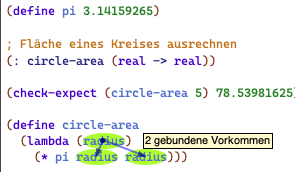
\includegraphics[width=0.5\textwidth]{i1hop/binding}
  \caption{Anzeige von Bindung nach Syntaxprüfung}
  \label{fig:binding}
\end{figure}

Die Beziehung zwischen den Bindung und gebundenen Vorkommen kannst
Du in DrRacket visualisieren, indem Du auf den Knopf
\texttt{Syntaxprüfung} (beziehungsweise \texttt{Check Syntax})
drückst und dann mit dem Mauszeiger über Variablenvorkommen
streichst.  Abbildung~\ref{fig:binding} zeigt exemplarisch, wie das aussieht.

\begin{aufgabeinline}
  Probiere die \texttt{Syntaxprüfung} auf dem Fußball-Code aus und
  untersuche zum Beispiel die Variablen in der Funktion
  \lstinline{home-points}.
\end{aufgabeinline}

Eine dritte Kategorie von Bindung gibt es auch noch, nämlich die
"<eingebauten"> Variablen wie \texttt{string-append} und
\lstinline{+}, die ähnlich global sichtbar sind wie die globalen
Variablen.  Wenn Du über sie nach \texttt{Syntaxprüfung} streichst,
wird \texttt{importiert aus} angezeigt.

Damit könnte man meinen, es sei alles zur Bindung gesagt: Globale und
eingebaute Variablen sind überall sichtbar; eine lokale Variable ist
innerhalb ihres \lstinline{lambda}-Rumpfes beziehungsweise
\lstinline{cond}-Zweiges sichtbar.  Aber was ist mit der folgenden
Funktion?
%
\begin{lstlisting}
(define f
  (lambda (x)
    (define y (+ x 1))
    (lambda (x)
      (+ x y))))
\end{lstlisting}
%
Die ist zugegeben künstlich konstruiert.  Aber wie verhält sie sich?
%
\begin{aufgabeinline}
  Was liefert die Auswertung von \lstinline{((f 1) 2)}?
\end{aufgabeinline}
%
In dieser Funktion gibt es \emph{zwei} Variablen namens \lstinline{x}:
Zwei Bindungen als Parameter und auch zwei gebundende Vorkommen.
Welche gebundenen Vorkommen gehören zu welchen Bindungen?  Hier gilt
die Regel der sogenannten \textit{lexikalischen Bindung}:
%
\begin{definition}[Lexikalische Bindung]\index{lexikalische Bindung}\index{Bindung!lexikalisch}
  Du findest die zu einem gebundenen Vorkommen zugehörige Bindung,
  indem Du von innen nach außen in der Klammerstruktur der Funktion
  suchst: Die erste Bindung als Parameter oder lokale Definition, die
  Du so findest, gehört zu dem gebundenden Vorkommen.

  Wenn Du auf diese Art und Weise keine Bindung findest, halte
  Ausschau nach einer globalen Definition.  Wenn Du keine globale
  Definition findest, muss es sich um eine eingebaute beziehungsweise
  importierte Definition handeln.
\end{definition}
%
Die lexikalische Bindung ordnet einer Bindung ihre gebundenden
Vorkommen zu.  Das bedeutet, dass Du, wenn Du eine Bindung und all
ihre gebundenen Vorkommen unbenennst, das Verhalten des Programms
nicht änderst.  Entsprechend sind also Variablen, die zu
unterschiedlichen Bindungen gehören, unterschiedliche Variablen.  Wenn
Du nach einer Syntaxprüfung über einer Variable das Kontextmenü
("<rechte Maustaste">) aufrufst, gibt es dort einen Punkt
\texttt{umbenennen}, der das Umbenennen automatisiert.

Der Begriff "<lexikalische Bindung"> suggeriert, dass es noch andere
Formen der Bindung gibt: Tatsächlich funktioniert Bindung in einigen
anderen, vornehmlich älteren Sprachen, nach anderen Prinzipien, oft
unter dem Begriff \textit{dynamische Bindung}\index{dynamische
  Bindung}\index{Bindung!dynamisch} zusammengefasst.  Lexikalische
Bindung wird oft auch \textit{statische Bindung}\index{statische
  Bindung}\index{Bindung!statisch} genannt.  "<Statisch"> bedeutet
im Kontext der Programmierung "<bevor das Programm läuft"> und
statische Bindung bedeutet, dass Du die Beziehung zwischen Bindungen
und gebundenen Vorkommen am Programmtext ablesen kannst.  Bei
dynamischer Bindung ergibt sich diese Beziehung erst, wenn das
Programm läuft.

Die Definition von \lstinline{f} kommt Dir vielleicht esoterisch vor.
Tatsächlich haben wir aber schon oft Programme geschrieben, bei denen
mehrere Variablen gleichen Namens auftauchen, wie zum Beispiel \lstinline{home-points}:

\begin{lstlisting}
(: home-points (game -> points))
...
(define home-points
  (lambda (game)
    ...))
\end{lstlisting}
%
Hier gibt es zwei Variablen namens \lstinline{game}: In der
Signaturdeklaration ist das die Signatur \lstinline{game} aus der
gleichnamigen Record-Definition.  In der Funktion ist es der Parameter
\lstinline{game}.  Dieser erfüllt die Signatur \lstinline{game}~--
darum haben die Signatur und der Parameter ja gerade den gleichen
Namen, um diese Beziehung deutlich zu machen.

Man könnte meinen, \emph{jetzt} wäre alles gesagt zur Bindung.  Aber
es gibt noch eine weitere Besonderheit, nämlich wenn in einer
Definition (gleich ob lokal oder global) die Variable, die definiert
wird, auch gleich wieder auftaucht.  Auch davon haben wir schon
ständig Gebrauch gemacht, nämlich in rekursiven Funktionen, wo für den
rekursiven Aufruf genau die Variable benutzt wird, in deren Definition
sie sich befindet.

\begin{aufgabeinline}
  Zu welchen Bindungen gehören die gebundenden Vorkommen von
  \lstinline{x} in folgendem Programm?
\begin{lstlisting}
(define g
  (lambda (x)
    (define x (+ x 1))
    (define y (+ x 1))
    (lambda (x)
      (+ x y))))
\end{lstlisting}
  Kannst Du vorhersagen~-- ohne es in der REPL auszuprobieren~-- was
  \lstinline{((g 1) 2)} liefert?
\end{aufgabeinline}


\section*{Aufgaben}

\begin{aufgabe}
  Schreibe eine Funktion \lstinline{any?}, die dann \lstinline{#t}
  zurückgibt, wenn mindestens ein Element der Liste das Prädikat
  erfüllt, sonst \lstinline{#f}.  Schreibe dann eine Funktion
  \lstinline{every?}, die dann \lstinline{#t} zurückgibt, wenn alle
  Elemente der Liste das Prädikat erfüllen, sonst \lstinline{#f}.
  Schreibe zunächst eine Fassung nach dem Muster von \lstinline{any?}.
  Schreibe eine zweite Fassung, die einfach \lstinline{any?} aufruft
  und selbst keine Rekursion benutzt.
\end{aufgabe}

\begin{aufgabe}
  Schreibe Funktionen \lstinline{feed-animals} und
  \lstinline{run-over-animals} die mit Hilfe der Funktionen in
  Abschnitt~\ref{sec:feed-animal} auf Seite~\pageref{sec:feed-animal}
  alle Tiere auf dem Highway (die sich in einer Liste befinden)
  füttert respektive überfährt.
\end{aufgabe}

\begin{aufgabe}
  Schreibe folgende Funktionen unter der  
  Verwendung von \lstinline{filter}!
  \begin{itemize}
    \item Schreibe eine Funktion \lstinline{evens}, welche die ungeraden Zahlen aus 
      einer Liste entfernt,
  \item eine Funktion \lstinline{count-zeroes}, die in einer Liste von
    Zahlen die Nullen zählt,
  \item und eine Funktion \lstinline{multiples}, die eine Zahl $n$ und
    eine Liste von Zahlen akzeptiert, und eine Liste alle Vielfachen
    der Zahl $n$ liefert.
  \end{itemize}
\end{aufgabe}

\begin{aufgabe}
  Programmiere eine Funktion
  \lstinline{filter-map}, die als Argumente eine Funktion \lstinline{p} mit
  einem Argument sowie eine Liste \lstinline{l} akzeptiert.
  \lstinline{Filter-map} soll als Ergebnis die Liste der Rückgabewerte
  von \lstinline{p} für diejenigen Elemente von \lstinline{l} zurückgeben,
  für die \lstinline{p} nicht \lstinline{#f} zurückgibt. Beispiel:

\begin{lstlisting}
(filter-map (lambda (x)
               (if (even? x)
                  (+ x 1)
                  #f))
            (list 1 2 5 17 24 13))
|\evalsto| #<list 3 25>
\end{lstlisting}
\end{aufgabe}

\begin{aufgabe}
  Verwende die Funktion \lstinline{list-fold} um folgende 
  Funktionen zu schreiben:
  \begin{enumerate}
  \item Schreibe eine Funktion \lstinline{list-map}, die eine Funktion auf jedes
    Element einer Liste anwendet.
  \item Schreibe eine Funktion \lstinline{list-or}, die ein Prädikat auf alle
    Elemente einer Liste anwendet und die Resultate mit \lstinline{or}
    verknüpft.
  \item Schreibe eine Funktion \lstinline{count-predicate}, die ein Prädikat auf
    alle Elemente einer Liste anwendet und zählt, wie häufig \lstinline{#t}
    zurückgegeben wird.
  \item Schreibe eine Funktion \lstinline{contains?}, die feststellt, ob ein
    Element in einer Liste enthalten ist.
  \item Schreibe eine Funktion \lstinline{remove-duplicates}, die alle doppelten
    Elemente aus einer Liste filtert.
  \end{enumerate}
\end{aufgabe}

\begin{aufgabe}
  Fußballreporter zitieren gern obskure Fakten über
  vergangene Spiele, wenn sie zum Spielverlauf wenig zu sagen haben.

  Hier ein Beispiel:
  % 
  \begin{quote}
    "<In der Saison 2009/2010 gab es ja immerhin vier Spieltage, an
    denen die größte Tordifferenz kleiner als 3 war.">
  \end{quote}
  %
\begin{enumerate}
\item Stelle dem Fußballreporter Hilfsfunktionen zur Verfügung,
  die ihm erlauben, eine Antwort auf solch eine Frage zu
  finden:
  %
  \begin{quote}
    \emph{An wie vielen Spieltagen der Saison 2009/2010 war die größte
    Tordifferenz kleiner als 3?}
  \end{quote}
  %
  Schreibe mit Hilfe dieser Funktionen einen Ausdruck, der
  testet, ob die am Anfang dieser Aufgabe zitierte Aussage über die
  Tordifferenzen in der Saison 2009/2010 stimmt!

  \begin{enumerate}
  \item Schreibe eine Funktion, die aus einer Liste die Dubletten
    entfernt.  Diese Funktion akzeptiert eine Liste sowie eine
    Funktion, die zwei Elemente der Liste akzeptiert und
    zurückliefert, ob diese gleich sind.  (Also zum Beispiel
    \lstinline{=} bei Listen von Zahlen.)  Sie liefert dann eine Liste,
    in der jedes Element "<nur einmal vorkommt">, also kein anderes,
    das dazu gleich ist.
  \item Schreibe eine Funktion, die aus der Liste aller Spiele
    eine Liste aller Spielplannummern extrahiert.
  \item Schreibe eine Funktion, die aus der Liste aller Spiele
    eine Liste von Listen aller Spiele macht~-- so dass in jeder
    Teilliste alle Spiele eines Spieltags zusammengefasst sind.
  \item Schreibe eine Funktion, welche die Tordifferenz eines
    Spiels zurückliefert.
  \item Schreibe eine Funktion, welche das maximale Element einer
    Liste berechnet.  Die Funktion sollte neben der Liste eine
    Funktion akzeptieren, die berechnet, ob ein Element "<kleiner oder
    gleich"> einem anderen ist.
  \item Schreibe schließlich einen Ausdruck, der die Anzahl der
    Spieltage der Saison 2009/2010 liefert, bei denen die größte
    Tordifferenz kleiner als 3 war.
  \end{enumerate}

  \item Schreibe Ausdrücke, die folgende Fragen beantworten~--
  entwickele dazu, falls nötig, weitere Hilfsfunktionen:
  \begin{itemize}
    \item An welchem Spieltag gab es die meisten Heimsiege?
    \item An welchem Spieltag fielen die meisten Tore?
    \item Gab es mehr Siege für die Heimmanschaften an ungeraden Spieltagen als an
      geraden?
    \end{itemize}
\end{enumerate} 

\end{aufgabe}

\begin{aufgabe}

  Betrachte das folgende Programm:

\begin{lstlisting}
(define x 2)          ;  --> zwei
(define y -1)         ;  --> minuseins
(define z -3)         ;  --> minusdrei

(define f 
  (lambda (x z)
    (+ (* x x) z y)))

(f 4 -2)
\end{lstlisting}
  %
  Benenne die Variablen \lstinline{x}, \lstinline{y} und \lstinline{z}, die in
  den ersten drei Zeilen des Programms definiert werden, im kompletten
  Programm um, und zwar \lstinline{x} in \lstinline{zwei}, \lstinline{y} in
  \lstinline{minuseins} und \lstinline{z} in \lstinline{minusdrei}. Achte bei
  der Umbenennung auf die lexikalische Bindung.  Benenne keine
  Parameter der Funktion \lstinline{f} um.

  Nachdem Du die Umbenennung durchgeführt hast, welches Ergebnis liefert
  der Ausdruck \lstinline{(f 4 -2)}? Berechne das Ergebnis von Hand mit Hilfe
  des Substitutionsmodells und halte die Zwischenschritte fest.
\end{aufgabe}

\begin{aufgabe}

  Betrachte das folgende Programm:

\begin{lstlisting}
(define x 2)                    ; --> zwei
(define y 4)                    ; --> vier

(define z                       ; --> f
  (lambda (x y z)
    (+ x (z y))))

(z y x (lambda (z) (+ x z)))
\end{lstlisting}
%
  Benenne die Variablen \lstinline{x}, \lstinline{y} und \lstinline{z}, die in
  den ersten drei Zeilen des Programms definiert werden, im kompletten
  Programm um. Der neue Name der Variable steht als Kommentar im
  Programm hinter dem Pfeil (\lstinline{-->}).  Achte bei der
  Umbenennung auf die lexikalische Bindung.  Benenne keine
  Parameter der Funktion \lstinline{z} um.

  Berechne, nachdem Du die Umbenennung durchgeführt haben, von
  Hand \lstinline{(z y x}
  \lstinline{(lambda (z) (+ x z))))} und halte die Zwischenschritte
  fest.

\end{aufgabe}

\begin{aufgabe}
  Betrachte folgendes Programm:

\begin{lstlisting}
(define x 1)
(define y 3)
(define z 5)

(define f
  (lambda (x)   
     ((lambda (y)
        ((lambda (z)
           (+ z (* x y)))
         (+ x z)))
      (+ x y))))

(f y)
\end{lstlisting}

  Benenne hier alle lokalen Variablen, die innerhalb der Funktion
  \lstinline{f} gebunden werden, um. Verändere nicht den Namen der
  Variablen \lstinline{x}, \lstinline{y} und \lstinline{z} aus den ersten drei Zeilen
  des Programms.

  Nachdem Du die Umbenennung durchgeführt haben, welches Ergebnis liefert
  der Ausdruck \lstinline{(f y)}? Berechne das Ergebnis von Hand mit Hilfe
  des Substitutionsmodells und halte die Zwischenschritte fest.

  \noindent \emph{Hinweis:} In diesen Aufgaben findest Du keine
  Kommentare und Signaturen zu den Funktionen. Hier kannst Du an einem
  Beispiel sehen, dass es sehr wichtig ist, diese Informationen
  anderen Programmierern immer zur Verfügung zu stellen. Denn es kann
  auch bei kleinen Programmen schwer sein, die Funktionsweise der
  einzelnen Funktionen ohne Kommentare zu verstehen.
\end{aufgabe}

\begin{aufgabe}
  Funktionen können nicht nur als Argumente an
  andere Funktionen übergeben, sondern auch als Ergebnisse
  zurückgeliefert werden. Dies soll in dieser Aufgabe genutzt werden,
  um ein einfaches Telefonbuch zu implementieren: Ein Telefonbuch ist
  als Funktion repräsentiert, die den Namen einer Person akzeptiert
  und die Telefonnummer der Person zurückliefert.

  \begin{enumerate}
  \item Definiere zunächst eine Signatur
    \lstinline{phonebook-result} für das Ergebnis des Nachschlagens in einem
    Telefonbuch. Ein solches Ergebnis ist entweder eine Telefonnummer
    oder ein Wert, der "<nicht gefunden"> darstellt,
    Die Signatur des Telefonbuchs ist  \lstinline{(string -> phonebook-result)}.
  \item Definiere einen Wert \lstinline{empty-phonebook}, der das leere
    Telefonbuch repräsentiert.
  \item Definiere eine Funktion namens
    \lstinline{add-to-phonebook}, welche ein Telefonbuch, einen Namen
    und eine Telefonnummer erwartet und das um den neuen Eintrag
    erweiterte
    Telefonbuch zurückliefert.
  \item Schreibe eine Funktion namens \lstinline{lookup-in-phonebook},
    welche ein Telefonbuch und einen Namen einer Person erwartet und die
    Nummer der Person im Telefonbuch nachschlägt und zurückliefert.
    Beispiele:
    \begin{itemize}
    \item \lstinline{(lookup-in-phonebook empty-phonebook "Hans")} liefert
      "<nicht gefunden">.
    \item \lstinline{(lookup-in-phonebook} \\
      \lstinline{    (add-to-phonebook empty-phonebook "Hans" "754829")}\\
      \lstinline{    "Hans")} \\
      liefert die Nummer 754829.
    \item \lstinline{(lookup-in-phonebook}\\
      \lstinline{    (add-to-phonebook empty-phonebook "Hans" "754829")}\\
      \lstinline{    "Lea")}\\
      liefert "<nicht gefunden">.
    \end{itemize}
  \end{enumerate}
\end{aufgabe}

\begin{aufgabe}
  Diese Aufgabe ist für Dich geeignet, falls Du das entsprechende
  Wissen aus der Mathematik besitzt:

  Ein Polynom ist eine Funktion von $\mathbb{R}$ nach $\mathbb{R}$ und
  hat folgende Form:
  \begin{displaymath}
    p(x) = a_0 +
    a_1 \cdot x + a_2 \cdot x^2 + \ldots + a_n \cdot x^n    
  \end{displaymath}
  %
  Ein Polynom wird also eindeutig durch die Koeffizienten $a_0$ bis
  $a_n$ bestimmt.

  \begin{enumerate}
   \item Schreibe die Datendefinition für Polynome.
   \item Programmiere eine Funktion \lstinline{polynomial+}, die
     zwei Polynome addiert.  Schreibe ggf.\ zutreffende Eigenschaften auf
     und überprüfe diese!
     
   \item Programmiere eine Funktion \lstinline{polynomial*}, die zwei Polynome 
     multipliziert. 
     Beispielsweise werden die Polynome $a_0+a_1 x$ und $b_0+b_1 x$ nach folgendem Schema multipliziert:
     \begin{eqnarray*}
     & &a_0 \cdot (b_0+b_1x) \\
     &+&a_1 x \cdot (b_0+b_1 x) \\ 
     &=&a_0b_0+a_0b_1 x + a_1b_0x + a_1b_1x^2
     \end{eqnarray*}	
     Schreibe ggf.\ zutreffende Eigenschaften auf und überprüfe diese!
   \item Schreibe eine Funktion \lstinline{polynomial-function}, die
     ein Polynom akzeptiert und eine Funktion liefert, die ein Polynom
     an einer bestimmten Stelle auswertet, also gerade der Funktion
     $p$ aus der Definition entspricht. 
   \item Die Ableitung eines Polynoms $p$ wie oben ist bekanntlich durch
     \begin{displaymath}
       p'(x) = a_1 + 2\cdot a_2 \cdot x + 3\cdot a_3\cdot x^2 + \ldots
       + n \cdot a_n \cdot x^{n-1}
     \end{displaymath}
     gegeben. Schreibe die Funktion
     \lstinline{polynomial-derivative}, die von einem gegebenen Polynom das abgeleitete Polynom
     berechnet.
 \end{enumerate}
\end{aufgabe}

\begin{aufgabe}
  Listen lassen sich nach verschiedenen Kriterien
  sortieren: zum Beispiel aufsteigend, absteigend, oder abhängig von
  einem Feld der Elemente.  So kann eine Liste von Fußballspielen nach
  der Gesamtanzahl der Tore, der Anzahl der Tore des Heimteams oder
  der Anzahl der Tore des Gästeteams oder der Anzahl der Tore der
  gewinnenden Mannschaft sortiert werden.  Die genaue Anordnung wird durch
  eine Operation festgelegt, die bestimmt, ob ein Elemente vor einem anderen
  stehen soll.

\begin{enumerate}
\item Schreibe eine Funktion, die eine Liste nach einem beliebigen
  Kriterium sortiert.  Die Funktion sollte folgende Signatur haben:

\begin{lstlisting}
(: list-sort ((%a %a -> boolean) (list-of %a) -> (list-of %a)))
\end{lstlisting}

  Das erste Argument ist eine Funktion, die eine \textit{Ordnung}
  realisiert, also zwei Elemente vergleicht, und \lstinline{#t}
  zurückliefert, falls sie schon in der richtigen Reihenfolge sind und
  \lstinline{#f}, falls nicht.  Zum Beispiel können \lstinline{<=} oder \lstinline{>=}
  für das Sortieren von Listen von Zahlen verwendet werden.
\item Benutze diese Funktion, um eine Liste von
  Fußballspielen nach den folgenden Kriterien zu sortieren:
  \begin{itemize}
  \item Gesamtanzahl der Tore,
  \item Anzahl der Tore der Heimmannschaft,
  \item Anzahl der Tore des Gastmannschaft oder
  \item Anzahl der Tore der
    gewinnenden Mannschaft
  \end{itemize}
\end{enumerate}
\end{aufgabe}

\begin{aufgabe}
  Folgen mit unendlicher Länge lassen sich als
  zusammengesetzte Daten mit zwei Komponenten repräsentieren: Dabei
  ist die erste Komponente das erste Element der Folge und die zweite
  eine Funktion ohne Parameter, die, wenn sie angewendet wird, eine Folge mit
  den restlichen Elementen ohne das erste liefert.
  Solche unendlichen Folgen heißen \textit{Streams}.
  Schreibe Daten- und Record-Definition für Streams!

  Hier ist eine Funktion, die einen Stream aus natürlichen Zahlen,
  angefangen bei einer Zahl $n$, liefert:
  % 
  \begin{lstlisting}
; Stream mit Zahlen ab n erzeugen
(: from (natural -> stream))
(define from
  (lambda (n)
    (make-stream n
                 (lambda () (from (+ n 1))))))
  \end{lstlisting}
  % 
  (Dabei ist angenommen, dass der Konstruktor der Record-Definition
  \lstinline{make-stream} heißt.)
  Zur Betrachtung von Streams ist folgende Funktion nützlich, welche
  die ersten $n$ Elemente eines Streams als Liste extrahiert:
  % 
  \begin{lstlisting}
; erste Elemente eines Streams in eine Liste extrahieren
(: stream-take (natural stream -> (list-of %a)))
(define stream-take
  (lambda (n stream)
    (if (= n 0)
        empty
        (cons (stream-first stream)
                   (stream-take (- n 1)
                                ((stream-rest-proc stream)))))))
   \end{lstlisting}
   % 
   (Dabei ist angenommen, dass die Selektoren für Streams
   \lstinline{stream-first} und \lstinline{stream-rest-proc} heißen.)
   \lstinline{Stream-take} lässt sich z.B.\ auf das Ergebnis von
   \lstinline{from} anwenden:
   % 
   \begin{lstlisting}
(stream-take 17 (from 4))
|\evalsto| #<list 4 5 6 7 8 9 10 11 12 13 14 15 16 17 18 19 20>
   \end{lstlisting}
   % 
   Programmiere einige intellektuelle Herausforderungen mit Streams!
   \begin{enumerate}
   \item Programmiere eine Funktion \lstinline{stream-drop}, die eine
     natürliche Zahl $n$ und einen Stream akzeptiert, und einen neuen
     Stream liefert, der aus dem alten durch Weglassen der ersten $n$
     Elemente entsteht:
     \begin{lstlisting}
(stream-take 17 (stream-drop 3 (from 4)))
|\evalsto| #<list 7 8 9 10 11 12 13 14 15 16 17 18 19 20 21 22 23>
     \end{lstlisting}
   \item Programmiere eine Funktion \lstinline{stream-filter} analog zu
     \lstinline{filter}:
     % 
     \begin{lstlisting}
(stream-take 10 (stream-filter odd? (from 1)))
|\evalsto| #<list 1 3 5 7 9 11 13 15 17 19>
     \end{lstlisting}
   \item Programmiere eine Funktion \lstinline{drop-multiples}, die 
     eine Zahl $n$ und einen Stream von Zahlen $s$ akzeptiert.
     \lstinline{Drop-multiples} soll einen Stream liefern, in dem
     gegenüber $s$  alle Vielfachen von $n$ entfernt wurden:
     % 
     \begin{lstlisting}
(stream-take 10 (drop-multiples 3 (from 1)))
|\evalsto| #<list 1 2 4 5 7 8 10 11 13 14>
     \end{lstlisting}
   \item Schreibe eine Funktion \lstinline{sieve}, die aus einem Stream
     von Zahlen all diejenigen Zahlen entfernt, die Vielfache von
     Vorgängern im Stream sind:
     \begin{lstlisting}
(stream-take 10 (sieve (from 2)))
|\evalsto| #<list 2 3 5 7 11 13 17 19 23 29>
     \end{lstlisting}
     Um was für Zahlen handelt es sich in dem Beispielaufruf und
     warum?
   \item Schreibe eine Funktion \lstinline{powers}, die für eine Zahl
     $n$ einen Stream ihrer Potenzen liefert:
     % 
     \begin{lstlisting}
(stream-take 10 (powers 2))
|\evalsto| #<list 2 4 8 16 32 64 128 256 512 1024>
     \end{lstlisting}
   \item Schreibe eine Funktion \lstinline{stream-map} analog zu
     \lstinline{list-map}:
     \begin{lstlisting}
(stream-take 10 (stream-map (lambda (x) (+ x 1)) (from 1)))
|\evalsto| #<list 2 3 4 5 6 7 8 9 10 11>
     \end{lstlisting}
   \item Schreibe eine Funktion \lstinline{merge}, die zwei
     aufsteigende Streams von Zahlen zu einem aufsteigenden Stream
     der Elemente beider Streams vereinigt:
     \begin{lstlisting}
(stream-take 10 (merge (powers 2) (powers 3)))
|\evalsto| #<list 2 3 4 8 9 16 27 32 64 81>
     \end{lstlisting}
   \item Schreibe eine Definition für einen Stream aufsteigend
     sortierter Potenzen von Primzahlen:
     \begin{lstlisting}
(stream-take 10 prime-powers)
|\evalsto| #<list 2 3 4 5 7 8 9 11 13 16>
     \end{lstlisting}
     Definiere dazu zunächst einen Stream aus Streams von Potenzen
     % 
     \begin{lstlisting}
(define prime-powers-stream (stream-map powers (sieve (from 2))))
     \end{lstlisting}
     % 
     Definiere eine Funktion \lstinline{merge-streams}, welche
     diesen Stream akzeptiert und die Elemente der Streams
     aus \lstinline{prime-powers-stream} mit Hilfe von \lstinline{merge}
     aufsteigend sortiert.
   \end{enumerate}
 \end{aufgabe}

 \begin{aufgabe}
  Betrachte folgende mysteriöse Funktion:
\begin{lstlisting}
(: // ((%a -> (%b -> %b)) (list-of %a) -> (%b -> %b)))

(define //
  (lambda (proc lis)
    (cond
      ((empty? lis)
       (lambda (y)
         y))
      ((cons? lis)
       (lambda (y)
         ((proc (first lis))
          ((// proc (rest lis))
           y)))))))
\end{lstlisting}
  % 
  \textbf{Hinweise:} Beachte die Signaturen! In mehreren
  Teilaufgaben gibt es Gelegenheiten, \lstinline{curry} bzw.\
  \lstinline{uncurry} zu benutzen.

  \begin{itemize}
  \item Vergleiche die Funktion mit \lstinline{list-fold} und
    beschreibe, wie \lstinline{//} und \lstinline{list-fold} zueinander
    in Beziehung stehen.  Schreibe, falls möglich, eine
    Definition von \lstinline{//}, die \lstinline{list-fold} benutzt und
    umgekehrt.
  \item Schreibe mit Hilfe von \lstinline{//} eine Funktion
    \lstinline{list-sum}, welche die Elemente einer Liste addiert.
  \item Schreibe eine Funktion \lstinline{insert}, die eine reelle
    Zahl $n$ akzeptiert und eine Funktion zurückliefert, die eine
    aufsteigend sortierte Liste von reellen Zahlen konsumiert und
    eine Liste zurückliefert, in der $n$ an die entsprechende
    Stelle der Liste einsortiert wurde.
  \item Schreibe mit Hilfe von \lstinline{//} eine Funktion, die
    eine Liste von reellen Zahlen aufsteigend sortiert.
  \end{itemize}
\end{aufgabe}


\begin{aufgabe}
  Betrachte folgendes mysteriöse Programm:
  % 
  \begin{lstlisting}
(define y
  (lambda (f)
    ((lambda (x)
       (f (lambda (z) ((x x) z))))
     (lambda (x)
       (f (lambda (z) ((x x) z)))))))

(define m
  (y
   (lambda (f)
     (lambda (x)
       (cond
         ((= x 1)
          1)
         ((> x 1)
          (* x (f (- x 1)))))))))
   \end{lstlisting}
  %
  Probiere \lstinline{m} aus~-- was macht die Funktion?  \lstinline{Y}
  wird auch \textit{Fixpunktkombinator}\index{Fixpunktkombinator}
  genannt.  Das Thema kommt in Abschnitt~\ref{sec:fixpunkt} auf
  Seite~\pageref{sec:fixpunkt} noch einmal ausführlich:
 \end{aufgabe}

\begin{aufgabe}
  Beweise, dass für Funktionen $p_1$ mit einem Parameter, die
  einparametrige Funktionen zurückgeben, und Funktionen $p_2$ mit zwei
  Parametern gilt:
  %
  \begin{center}
    \lstinline{(curry (uncurry $p_1$))} $=$ $p_1$\\
    \lstinline{(uncurry (curry $p_2$))} $=$ $p_2$
  \end{center}
 \end{aufgabe}

\begin{aufgabe}
  Eine Funktion $f$ ist \textit{idempotent}\index{idempotent}, wenn gilt:

  \begin{center}
    \lstinline{(compose $f$ $f$) $=$ $f$}
  \end{center}

  Zeige, dass folgende Funktion idempotent ist:

  \begin{lstlisting}
    (define abs
      (lambda (x)
         (if (negative? x)
             (- x)
             x)))  \end{lstlisting}

  Welche anderen idempotente Funktionen kennst Du?
\end{aufgabe}

%%% Local Variables: 
%%% mode: latex
%%% TeX-master: "i1"
%%% End: 
